\section{Rational Proofs for Space Bounded Computation}

\begin{frame}{One More Approach to Build Rational Proofs} % WIP
	\begin{itemize}[<+- | alert@+>]
		\item Scoring rules don't distinguish between different ``amounts of work''
		\item In fact, doing nothing gets you a fairly good reward (earlier example)
	\end{itemize}
	\onslide<+->
	\begin{block}{Another idea: ``Weak'' Interactive Proofs [BCEJKL08,AM13,CG15,CG17]}
		\begin{itemize}[<+- | alert@+>]
			\item Fix a reward $R^*$;
			\item Run an interactive protocol that returns \textsf{accept} or \textsf{reject}.
			\item Pay $R^*$ if it returns \textsf{accept}; $0$ otherwise.
		\end{itemize}
	\end{block}
	\onslide<+->
	We only need the \textit{test} to recognize a false answer with some ``not too small'' probability $\delta$.
	\onslide<+->
	
	\[
		 \expectation[\tilde{R}] \leq R^*(1-\delta)
	\]
	
\end{frame}

\begin{frame}{Rational Proofs for Bounded Space}
	\begin{block}{Theorem (informal)}
		If $L$ can be decided in time $T$ and space $S$ by a $DTM$, then it admits a rational proof with $O(\log T)$ rounds, $S \log T$ communication complexity and Verifier's running time.
	\end{block}
	\begin{itemize}[<+->]
		\item If $T=poly(n)$ and $S=polylog(n)$ then we have a $O(\log n)$ round protocol with a polylog verifier.		
	\end{itemize}
\end{frame}

\begin{frame}{Main Idea: Exploit the Configuration Graph}
	
	\begin{figure}
		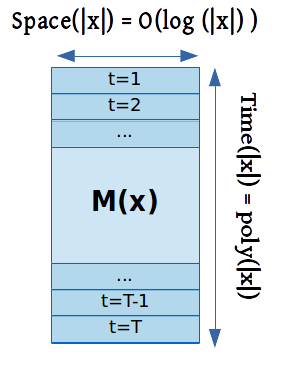
\includegraphics[scale=0.5]{pics/tm-rectangle.png}
	\end{figure}
	\begin{figure}
		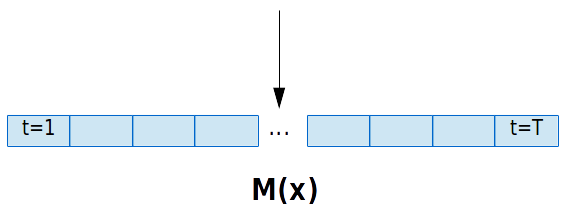
\includegraphics[scale=0.5]{pics/tm-lin.png}
	\end{figure}
\end{frame}

% r0
\begin{frame}{Execution Example}
	\begin{figure}
		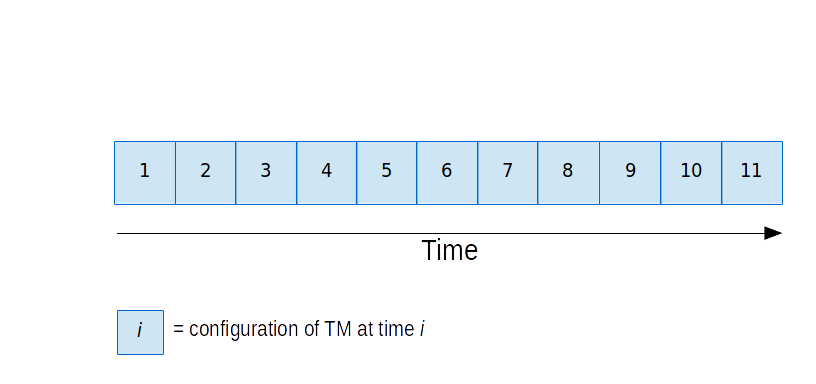
\includegraphics[scale=0.4]{pics/r0.png}
	\end{figure}
\end{frame}

%r1
\begin{frame}{Execution Example (cont.d)}
	\begin{itemize}
		\item $P$ sends $V$ the initial and final configurations .
	\end{itemize}
	\begin{figure}
		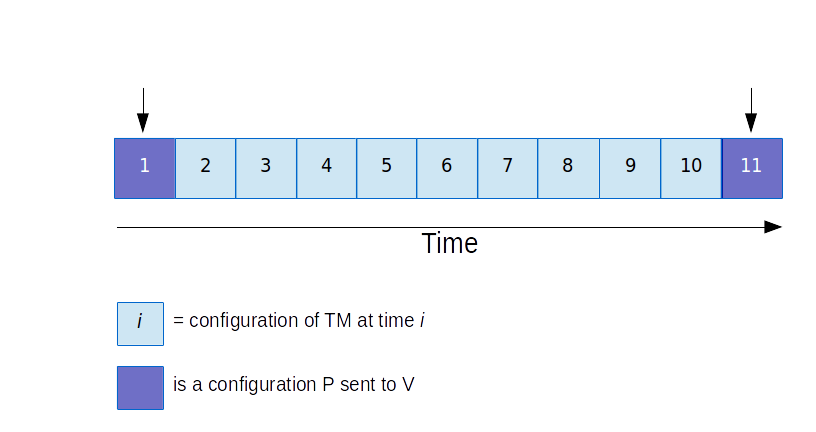
\includegraphics[scale=0.4]{pics/r1.png}
	\end{figure}
\end{frame}

%r2
\begin{frame}{Execution Example (cont.d)}
	
	\begin{itemize}
		\item $P$ sends $V$ the "midpoint" configuration (i.e. 6)
	\end{itemize}
	\begin{figure}
		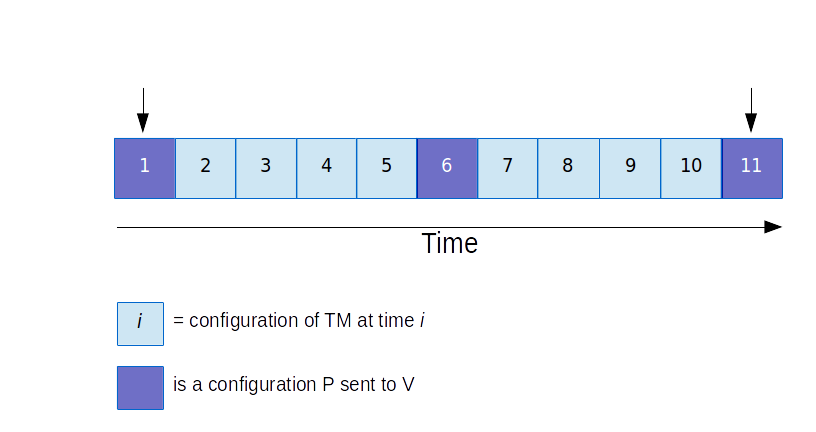
\includegraphics[scale=0.4]{pics/r2.png}
	\end{figure}
	
\end{frame}


%r2bis
\begin{frame}{Execution Example (cont.d)}
	\begin{itemize}
		\item $V$ flips a coin $b \in \{ 0,1 \}$. E.g. if $b = 0$, now the "window" of configurations shifts on the left half of the current window.
	\end{itemize}
	\begin{figure}
		
		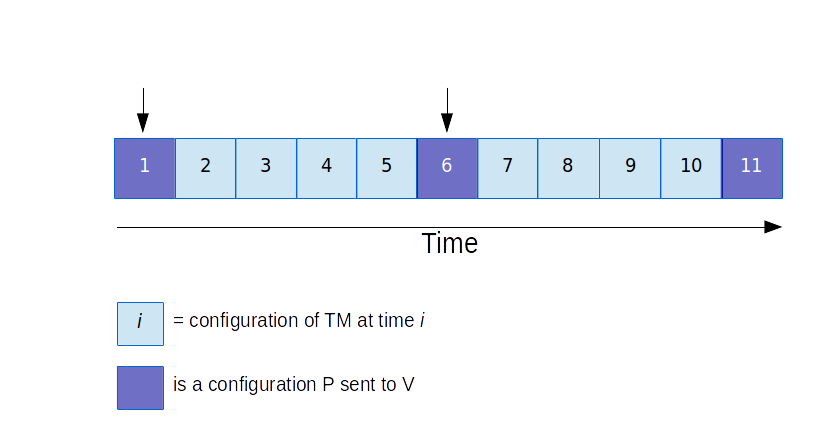
\includegraphics[scale=0.4]{pics/r2bis.png}
	\end{figure}
\end{frame}

%r3
\begin{frame}{Execution Example (cont.d)}
	\begin{itemize}
		\item $P$ sends $V$ the "midpoint" configurations (i.e. 3 and 4)
	\end{itemize}
	\begin{figure}
		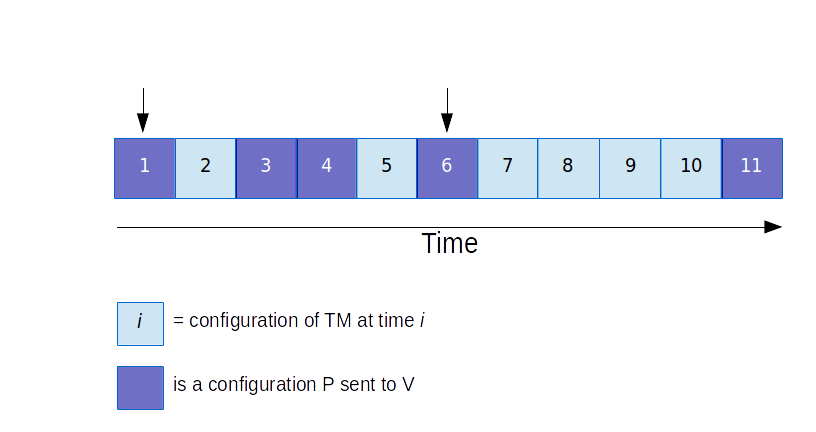
\includegraphics[scale=0.4]{pics/r3.png}
	\end{figure}
\end{frame}


%r3bis
\begin{frame}{Execution Example (cont.d)}
	\begin{itemize}
		\item $V$ flips a coin $b \in \{ 0,1 \}$. E.g. if $b = 1$, now the "window" of configurations shifts on the right half of the current window.
	\end{itemize}
	\begin{figure}
		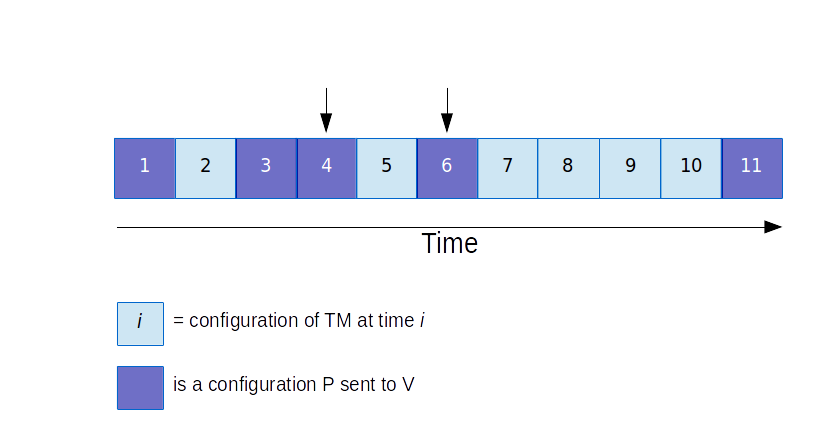
\includegraphics[scale=0.4]{pics/r3bis.png}
	\end{figure}
\end{frame}


%r-final
\begin{frame}{Execution Example (cont.d)}
	\begin{itemize}
		\item Now $V$ can check by itself that the transitions were consistent.
		\item $P$ receives reward $R$ only if final transition is consistent.
	\end{itemize}
	\begin{figure}
		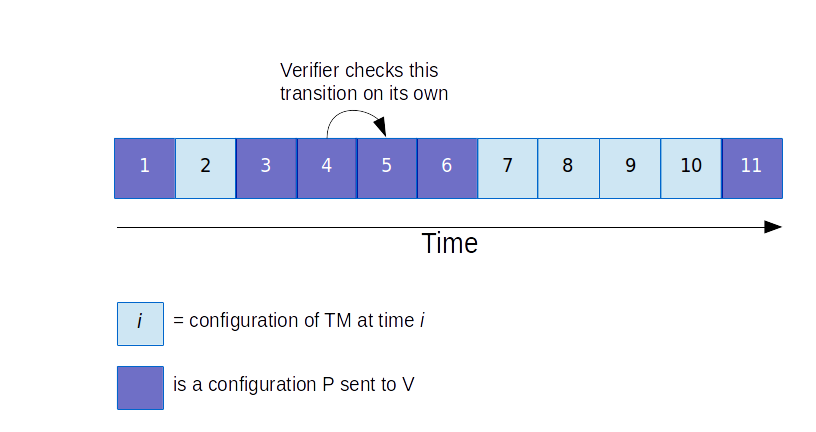
\includegraphics[scale=0.4]{pics/r-final.png}
	\end{figure}
\end{frame}


\begin{frame}{Analysis}
	\begin{block}{Efficiency}
	\begin{itemize}[<+- | alert@+>]
		\item The number of rounds is $O(\log T)$
		\item The Verifier's running time is $O(S \log T)$
	\end{itemize}
	\end{block}
	\onslide<+->
	\textbf{Rationality:} If the Prover cheats even on one transition it will lose in expectation a polynomial fraction of the honest reward.
	\onslide<+->
%	
%	\begin{block}{Sequential Composability (Intuition)}
%		\begin{itemize}[<+- | alert@+>]
%			\item If you haven't done all the work, then you are taking some risks in being found out;
%			\item The probability of being found out is proportional to the amount of work you haven't done;
%			\item Thus you'd be better off doing all the work.
%		\end{itemize}
%	\end{block}
%	\onslide<+->
%	\textbf{Caveat:} For that logic to work we need one more assumption.
\end{frame}

\begin{frame}{Sequential Composability (Intuition)}
		\begin{block}{Lemma (informal):}
			To achieve sequential composability it is sufficient to detect a cheating prover that invests $\tilde{C}$ with probability at least $\frac{\tilde{C}}{C^*}$

		\end{block}
	
		\onslide<+->
		\begin{block}{In the Last Protocol:}
		\begin{itemize}[<+- | alert@+>]
			\item If you haven't done all the work, then you are taking some risks in being found out;
			\item The probability of being found out is proportional to the amount of work you haven't done;
			\item Thus you'd be better off doing all the work.
		\end{itemize}
		\end{block}
	\onslide<+->
	\textbf{Caveat:} For that logic to work we need one more assumption.
\end{frame}

\begin{frame}{An Assumption on Cost}
		\begin{block}{}
		Investing at most a fraction $\gamma$ of the ``honest'' cost $\implies$ guessing $f(x)$ has probability at most\footnote<1->{plus some additive factor.} $\gamma$ 
	\end{block}
	
	\onslide<+->
	\begin{block}{Our results depend on this assumption. When does it hold?}
	\end{block}
	\onslide<+->
	\begin{itemize}[<+- | alert@+>]	
		\item It is unlikely interesting functions and distributions would satisfy \textit{directly} this assumption. (e.g. n-ary $\mathsf{AND}$).
		\item One option would be compiling $f$ into $\hat{f}$ where the assumption holds.
		\begin{itemize}
			\item possibly using approaches such as randomized encodings [IK00], proofs of useful work [BRSV17];
			\item \textbf{Left as future work.} (and not necessarily included in thesis).
			
		\end{itemize}
		\item \textbf{Next:} An alternative approach.
	\end{itemize}
	
\end{frame}